\documentclass[a4paper]{article}

\usepackage[spanish]{babel}
\usepackage{listings}
\usepackage[utf8]{inputenc}
\usepackage{titling}
\usepackage{enumitem}
\usepackage{fancyhdr}
\usepackage{xcolor}
\usepackage{geometry}
\usepackage{graphicx}
\usepackage{hyperref}
\geometry{a4paper, margin=7em}


\lstset{
    frame=single,
    breaklines=true,
    numbers=left,
    keywordstyle=\color{blue},
    numbersep=15pt,
    numberstyle=,
    basicstyle=\linespread{1.5}\selectfont\ttfamily,
    commentstyle=\color{gray},
    stringstyle=\color{orange},
    identifierstyle=\color{green!40!black},
}

%%\setlength{\parindent}{4em}
\setlength{\parindent}{0em}
\setlength{\parskip}{0.8em}
    
%%\renewcommand{\familydefault}{phv} %%Seleccionamos Helvetica
    
\lstdefinestyle{console}
{
    numbers=left,
    backgroundcolor=\color{violet},
    %%belowcaptionskip=1\baselineskip,
    breaklines=true,
    %%xleftmargin=\parindent,
    %%showstringspaces=false,
    basicstyle=\footnotesize\ttfamily,
    %%keywordstyle=\bfseries\color{green!40!black},
    %%commentstyle=\itshape\color{green},
    %%identifierstyle=\color{blue},
    %%stringstyle=\color{orange},
    basicstyle=\scriptsize\color{white}\ttfamily,
}
    
\title{Mapa de memoria}
\author{Aldán Creo Mariño}
    
    
\pagestyle{fancy}
\fancyfoot[R]{\thepage}
\fancyfoot[C]{}
\makeatletter
\let\runauthor\@author
\let\runtitle\@title
\makeatother
\fancyhead[L]{\runauthor}
\fancyhead[C]{SOI}
\fancyhead[R]{Práctica 5}
    
\begin{document}
%%\maketitle

\section{Mapa de memoria}

El siguiente mapa de memoria se produce cuando enlazo dinámicamente\footnote{Estoy usando {\ttfamily cat} porque es el método sugerido, pero también se puede acceder al mapa de memoria usando {\ttfamily pmap}.}:

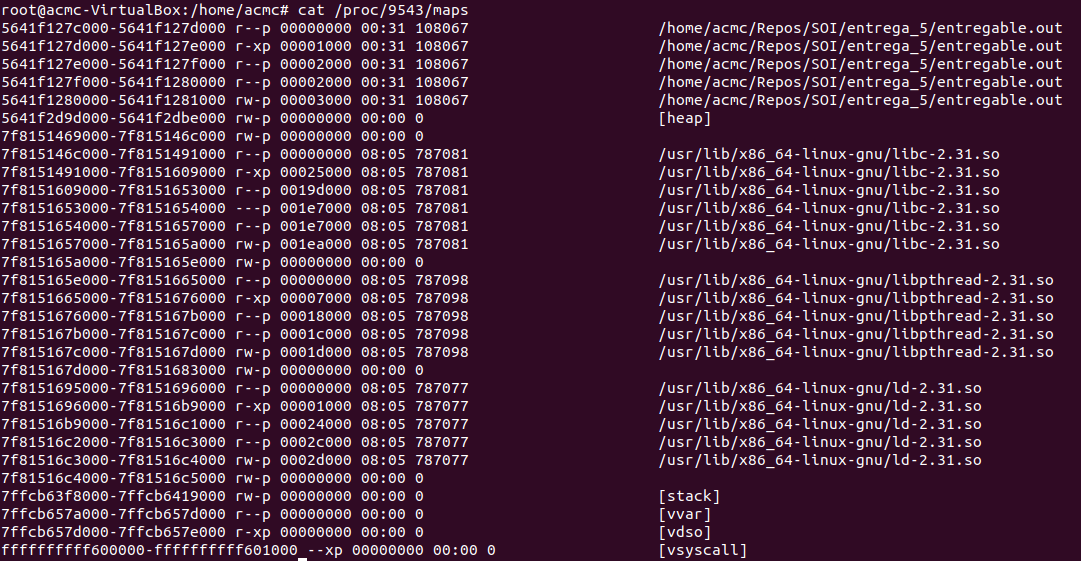
\includegraphics[scale=0.421]{6_padre.png}

Lo que significa cada columna ya se indica en el material de la práctica, así que por cuestión de espacio no lo voy a repetir. En este proceso, todas las regiones son privadas, y eso es lógico, ya que no queremos compartir ningún segmento de memoria con otro(s). Para ser breve, no haré referencias a este dato durante este informe, pero es relevante comentarlo, ya que podría interesar que haya secciones \emph{shared}.

\subsection{Variables globales}

Las variables globales se guardan en el segmento de datos ({\ttfamily.data}, si están inicializadas, o si no, en {\ttfamily.bss}). En el mapa de memoria del proceso, corresponderán con la sección con permisos de lectura y escritura, pero no ejecución, que se mapea al archivo del código (línea 5).

\subsection{Variables locales}

Las variables locales se guardan en el stack. Cuando se entra en una función, el compilador de C incluye código para decrementar el stack pointer, y guardar en el espacio que se ``crea'' (no en el mapa de memoria, sino que me refiero al espacio que queda libre al decrementar el puntero) las variables locales. Cuando se sale de la función, se incrementa el puntero, ``liberando'' en cierto modo la memoria.

Esto, en el mapa de procesos, se encuentra en la zona que se denota con la etiqueta {\ttfamily [stack]} (zona elevada de memoria, aunque la dirección exacta es aleatoria\footnote{Esto es así por cuestiones de seguridad: se evita que la posición en memoria de las secciones del programa se pueda conocer a priori. Más sobre esta cuestión en \href{https://manybutfinite.com/post/anatomy-of-a-program-in-memory/}{este artículo}.}). Lógicamente, tiene permisos {\ttfamily rw-p}. Podemos leer y escribir, pero no ejecutar, en esa zona.

El stack es el único segmento de memoria en el que, si se produce una referencia a memoria que no está dentro del segmento, pero sí dentro de su máximo total (usualmente unos 8MB), el sistema incrementa automáticamente su tamaño, en vez de lanzar un fallo de segmento (el comportamiento normal)\footnote{Como se indica en \href{https://stackoverflow.com/questions/54564273/dynamic-expansion-of-the-linux-stack}{este enlace}, el kernel decide si lanzar un fallo de segmento o aumentar el tamaño de este segmento comprobando el valor actual del stack pointer.}. Esto es para permitir el crecimiento natural del {\ttfamily stack} con las llamadas a rutinas.

\subsection{Memoria dinámica}

La memoria dinámica es un concepto algo más complejo. Voy a hablar de las funciones de la familia {\ttfamily malloc}, aunque siendo estrictos podríamos gestionar la memoria dinámica nosotros mismos.

La gestión de la memoria se basa en el mapeo de direcciones de memoria arbitrariamente grandes a segmentos con permisos de lectura y escritura. Es decir, se trata de pedir al sistema regiones de memoria en las que poder trabajar con datos. {\ttfamily malloc} implementa esta idea a través de dos vías:
\begin{itemize}
    \item Usando memoria del {\ttfamily heap}. Si la memoria que le pedimos a {\ttfamily malloc} es relativamente pequeña, llegará con aumentar el tamaño del {\ttfamily heap} con la llamada al sistema {\ttfamily brk}.
    \item Si el tamaño que pedimos a {\ttfamily malloc}, en cambio, es mayor que {\ttfamily MMAP\_THRESHOLD} (valor configurable con la función {\ttfamily mallopt}), entonces {\ttfamily malloc} usa la llamada al sistema {\ttfamily mmap}, para crear un nuevo segmento en el que 
\end{itemize}

\subsection{Creando nuevos hilos}

Si creamos un hilo, vemos que aparece la siguiente línea en el mapa:

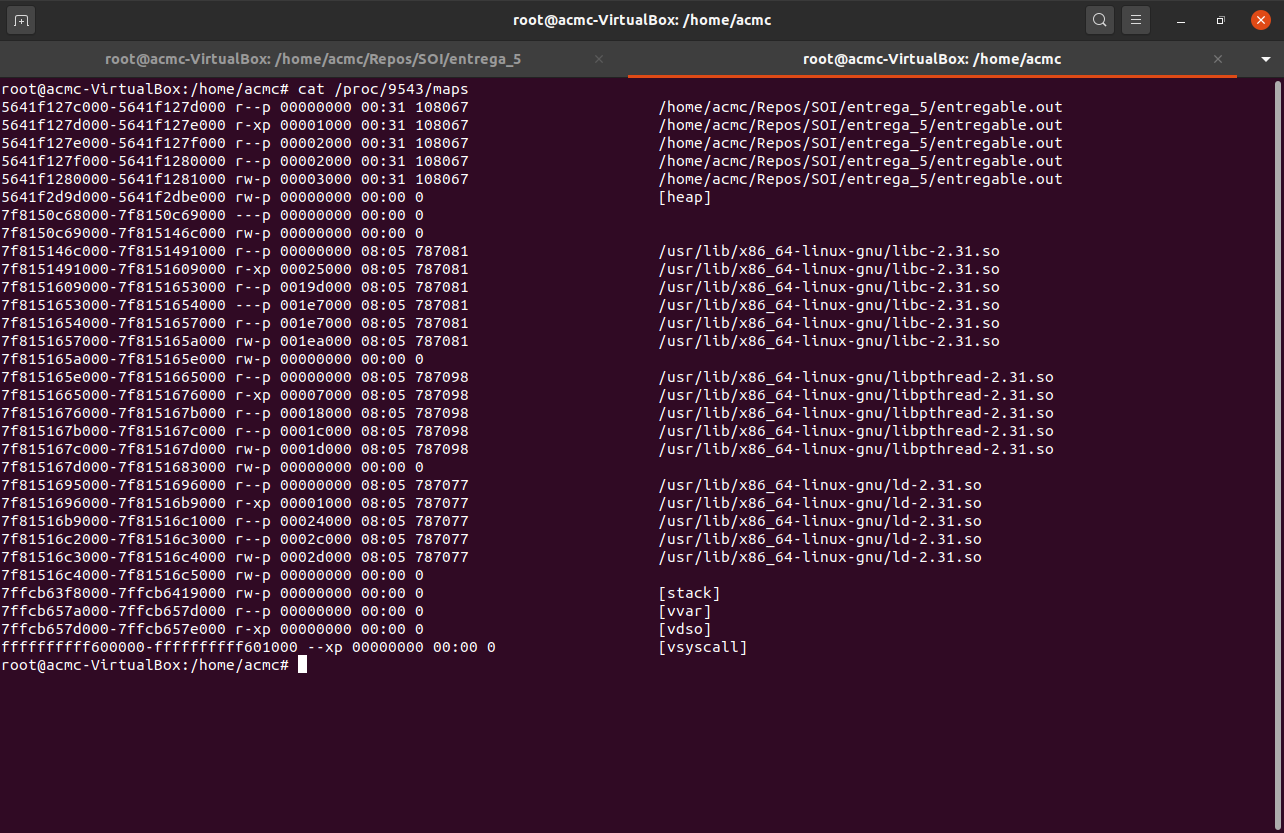
\includegraphics[scale=0.447]{6_hijo1.png}

Esto se corresponde con el stack para el nuevo hilo. En las prácticas optativas pude usar la función {\ttfamily clone()}, que deja ver de forma bastante más expícita la necesidad de crear un stack para el hilo. En el caso de la llamada a {\ttfamily clone()}, primero es necesario reservar manualmente un espacio en la memoria para alojar el stack del nuevo hilo. Esto se hace usando {\ttfamily malloc}, que se encargará de reservar una zona de memoria que aloje el stack. Al llamar a {\ttfamily pthread\_create}, este segmento de memoria se mapea de forma implícita.

En el mapa de memoria, el mapeo de esta entrada es anónimo, porque no se corresponde con ningún archivo, sino que es un segmento que se crea en tiempo de ejecución y sólo está dentro de este proceso.

Si creo el segundo hilo, aparece otro segmento para reservar su stack:

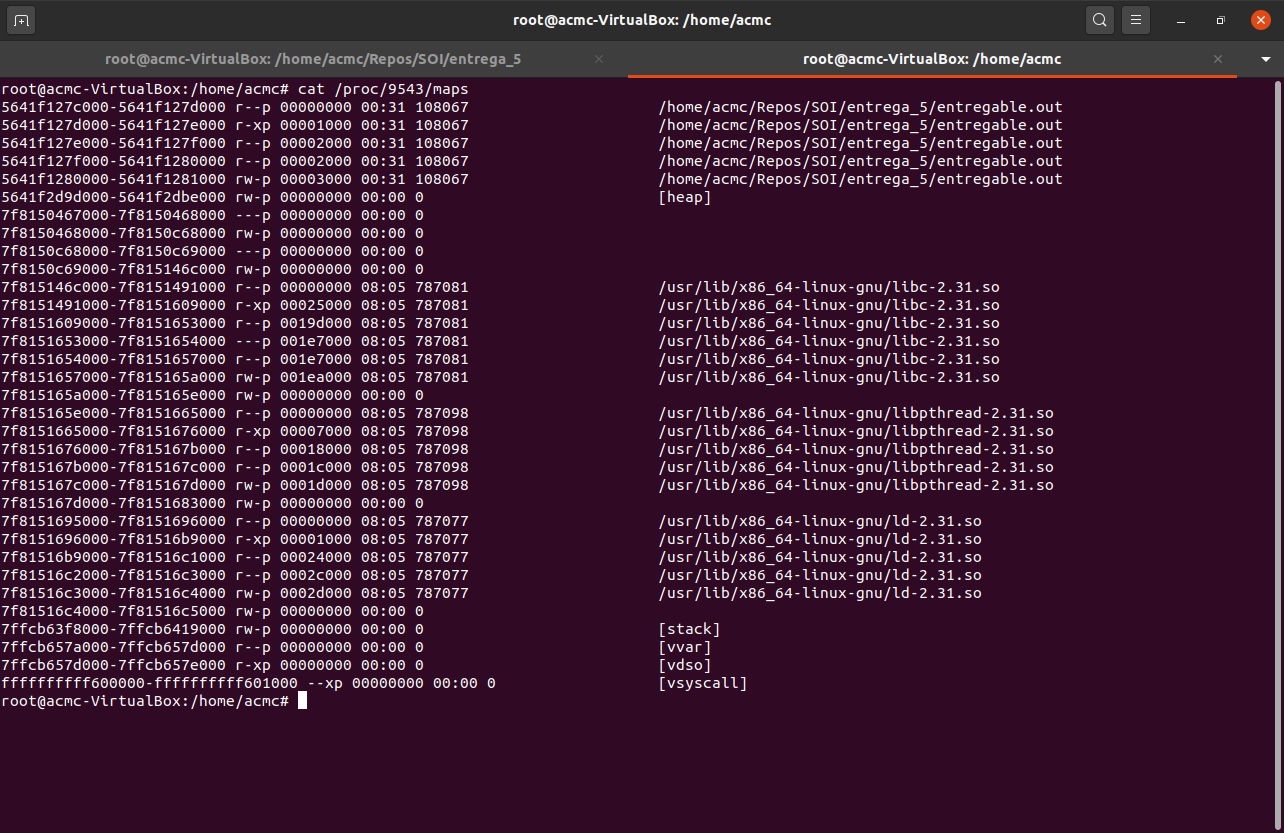
\includegraphics[scale=0.408]{6_hijo2.png}

Las entradas que figuran en el mapa que no tienen ningún tipo de permiso tienen el propósito de servir como protección. Básicamente, están ahí para que, en caso de que intentemos escribir o leer en ellas, tengamos un segmentation fault (ya que no deberíamos poder). Esto es lógico si pensamos que el stack puede crecer hasta desbordarse. Si se desborda, en este caso se desbordaría hacia estos segmentos en los que no tenemos permisos, por lo que tendríamos el fallo de segmento que comentaba. Y eso es algo deseable, porque la otra opción sería no tener esos segmentos ``de proteción'' por el medio. En ese caso, podría haber dos situaciones:
\begin{itemize}
    \item Si la memoria no estuviera mapeada, e intentásemos acceder a ella, seguiríamos teniendo un segmentation fault, así que en ese caso no cambia nada.
    \item Si resultase que justo de forma contigua al segmento del stack hubiera otro segmento mapeado (por ejemplo, podría ser el stack de otro hilo), ¡podríamos escribir en el stack del otro hilo!
    
    Claramente, esto plantearía un serio problema de protección. Nuestro programa podría sufrir errores gravísimos si algo así sucediera. Por eso es mejor curarnos de males y tener estos segmentos ``de seguridad''. Técnicamente no eliminamos la posibilidad de direccionar a un segmento que no es el deseado, pero si combinamos esta técnica con la de la aleatorización de direcciones, tenemos un ambiente en el que es mucho más difícil que se produzcan esta clase de fallos en la memoria.
\end{itemize}

\subsection{{\ttfamily [vsyscall]}}

Es curioso comentar la última línea del mapa de memoria, ya que corresponde a una dirección que no está en el espacio de usuario. El espacio de usuario solo llega hasta {\ttfamily 0x7fffffffffff} \footnote{Se puede consultar \href{https://www.kernel.org/doc/Documentation/x86/x86_64/mm.txt}{este enlace} para obtener más detalles al respecto.}. Este segmento aparece reflejado en el mapa de memoria, porque se utilizaba para hacer llamadas al sistema de forma directa \footnote{Hoy en día, solo se mantiene por temas de compatibilidad. En \href{https://lwn.net/Articles/446528/}{este artículo} se comenta en detalle el funcionamiento de esta entrada del mapa.}. También es el uso de {\ttfamily [vdso]}, que se encuentra dentro del espacio de usuario para permitir la aleatoriedad de las direcciones (por los motivos de seguridad que comentaba al principio del informe)\footnote{{\ttfamily [vvar]} complementa la funcionalidad de {\ttfamily [vdso]}. También se comenta en el artículo anterior.}.

\subsection{Enlazado estático}

Por defecto, el enlazador de \emph{gcc} utiliza el enlazado dinámico. Esto es porque el enlazado dinámico ofrece varias ventajas, entre las que destaca especialmente el hecho de que reduce considerablemente el tamaño de los ejecutables. Pese a todo, si en vez de compilar el código del entregable de la forma estándar (enlazado dinámico), se compila especificando la opción {\ttfamily -static}, entonces el enlazado será estático, y esto implica que el código de las librerías que incluímos en nuestro programa se incluirá directamente en el código ejecutable. Esto implica un incremento considerable de tamaño (en mi caso, pasé de los 17kB a 1,6MB).

En el mapa de memoria, también se verá reflejado dicho cambio:

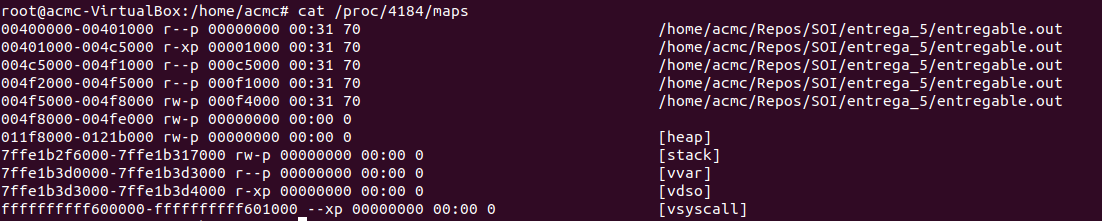
\includegraphics[scale=0.408]{Captura_estatico.png}

Aquí lo que vemos es que su número de entradas ha bajado mucho. Esto es porque todo el código de las librerías, que antes se mapeaba en el proceso, cargando el código desde los propios archivos de las librerías (en el primer mapa, se cargaba desde {\ttfamily libc-2.31.so}, {\ttfamily libpthread-2.31.so} y {\ttfamily ld-2.31.so}).

\end{document}